% Using a4paper and 12pt font by default
\documentclass[12pt, a4paper]{article}

%Includes "References" in the table of contents
\usepackage[nottoc]{tocbibind}

% Use more than one optional parameter in a new commands
\usepackage{xargs}

% Coloured text etc.
\usepackage[pdftex,dvipsnames]{xcolor}

% Pictures and /includegraphics
\usepackage{graphicx}
% Links in the table of contents + other stuff
\usepackage[hidelinks, linktoc=all]{hyperref}

% Support multi-page code listings
\usepackage[all]{hypcap}
\usepackage{subcaption}

% Times New Roman font
\usepackage[T1]{fontenc}
\usepackage{newtxmath,newtxtext}

% Margins
\usepackage[margin=2.5cm]{geometry}

% Interline
\usepackage{setspace}
\setstretch{1.5}

% Footnotes
\usepackage[bottom]{footmisc}

% Captions
\usepackage{caption}

% Todo notes
\usepackage[colorinlistoftodos,prependcaption,textsize=tiny]{todonotes}
\newcommandx{\unsure}[2][1=]{\todo[linecolor=red,backgroundcolor=red!25,bordercolor=red,#1]{#2}}
\newcommandx{\change}[2][1=]{\todo[linecolor=blue,backgroundcolor=blue!25,bordercolor=blue,#1]{#2}}
\newcommandx{\info}[2][1=]{\todo[linecolor=OliveGreen,backgroundcolor=OliveGreen!25,bordercolor=OliveGreen,#1]{#2}}
\newcommandx{\improvement}[2][1=]{\todo[linecolor=Plum,backgroundcolor=Plum!25,bordercolor=Plum,#1]{#2}}

% Code highlighting
\usepackage{minted}
\usemintedstyle{tango}
\newcommandx{\listcode}[2][1=]{\bgroup\inputminted[linenos, breaklines=true, fontsize=\scriptsize]{python}{#1}\captionof{listing}{#2}\egroup}
\newcommandx{\listcodecont}[2][1=]{\bgroup\inputminted[linenos, breaklines=true, fontsize=\scriptsize,firstnumber=last]{python}{#1}\captionof{listing}{#2}\egroup}

% New line after paragraph title
\newcommandx{\myparagraph}[1]{\paragraph{#1}\mbox{}}

% List stuff easily
\usepackage{multicol}
\usepackage[sharp]{easylist}

\let\OldEasylist\easylist
\let\OldEndEasylist\endeasylist
\renewenvironment{easylist}{%
    \OldEasylist%
    \ListProperties(Progressive*=3ex, Start1=1)%
}{%
    \OldEndEasylist%
}%


\begin{document}

% Title page

\begin{titlepage}
\end{titlepage}

\newpage

% Table of Contents

\tableofcontents

\newpage
% Misc
\newpage
\listoftodos[Temporary Notes]

% Abstract

\begin{abstract}

\end{abstract}



%===============================================================================
\newpage
\section{INTRODUCTION}
%===============================================================================

%-------------------------------------------------------------------------------
\subsection{State of the Art in Data Science}
%-------------------------------------------------------------------------------
\improvement[inline]{Use stuff from the presentation}
\begin{easylist}
# Why is data analysis useful?
## Modern amounts of data explanation
## Data analysis explanation
# What tools are used to deal with large amounts of data?
## Traditional - ETL and DW (microsoft, qlikview, ...)
## Explorational - spark, R, python, matlab
# Why choose python?
## Advantages and disadvantages of using python
## Overview of chosen packages
\end{easylist}

\change[inline]{Rewrite everything}
%-------------------------------------------------------------------------------
\subsection{Goals of the Research}
%-------------------------------------------------------------------------------
 In the modern world, big data and machine learning are becoming more and more prominent as companies such as Facebook, Google and Amazon gather and analyze all sorts of data from their users. But which tools are they using to do it?

Right now, the two main languages in data science are \mintinline{python}{Python} and \mintinline{python}{R}, while \mintinline{python}{Matlab} is also quite popular despite only being used in the academic environment.

This work's objective is to show how to use the Python 3 programming language in dealing with different kinds of data, and to help clarify any problems that might come up. It may be useful for long-term users of other languages that want to try Python out as well as users of Python 2, support for which will be stopped in 2020.
%-------------------------------------------------------------------------------
\subsection{Thesis Overview}
%-------------------------------------------------------------------------------
This work will be split into three parts, each working with a different dataset.

In the first part, I'll show you how to obtain, plot and predict stocks based on the last 17 years' worth of stock data from NYSE\footnotemark. I'll also cover some common problems that might occur when one is trying to deal with such amount of data.
\footnotetext{New York Stock Exchange}

In the second part, I'll cover scraping facebook's API, and plotting geolocation data of their events. I'll also discuss some problems that might occur while trying to download data, as well as how to use latest tools from Python (like the asyncio library) to speed up the data gathering part greatly. I'll also give you a brief overview of the current data visualization landscape, and show you which plotting packages are the best to use when dealing with geolocation data.

In the third part, I'll delve into the YouTube system, and will try to download and analyze their videos.

Lastly, the fourth part will contain conclusions.

%===============================================================================
\newpage
\section{TABULAR DATA ANALYSIS}
%===============================================================================
%-------------------------------------------------------------------------------
\subsection{Project Overview}
%-------------------------------------------------------------------------------
\begin{easylist}
# Goals
## Describe the project
# Obtaining the data (pandas-datareader)
# Traditional stock visualizations (matplotlib)
# Stock correlation matrix (matplotlib)
# LSTM training (keras)
\end{easylist}

%-------------------------------------------------------------------------------
\newpage
\subsection{Data gathering (pandas-datareader)}
%-------------------------------------------------------------------------------

%-------------------------------------------------------------------------------
\newpage
\subsection{Traditional stock visualizations (matplotlib)}
%-------------------------------------------------------------------------------

%-------------------------------------------------------------------------------
\newpage
\subsection{Stock correlation matrix visualization (matplotlib)}
%-------------------------------------------------------------------------------

%-------------------------------------------------------------------------------
\newpage
\subsection{Predictive analysis with a LSTM neural network (keras)}
%-------------------------------------------------------------------------------



%===============================================================================
\newpage
\section{GRAPH DATA ANALYSIS}
%===============================================================================
%-------------------------------------------------------------------------------
\subsection{Project Overview}
%-------------------------------------------------------------------------------
\begin{easylist}
# Goals
## to show how to run community detection algorithms in igraph
## to show how to plot the communities using two different methods - datashader  (larger data) and cairo (smaller data)
## to show how to make the communities visually separatable and how to incorporate node weights in the plot
# Tools(Libraries) used
## Why I chose igraph
\end{easylist}

\myparagraph{Packages needed}
\begin{easylist}
  # igraph
  # cairocffi
\end{easylist}

%-------------------------------------------------------------------------------
\newpage
\subsection{Preprocessing and igraph creation}
%-------------------------------------------------------------------------------
\begin{easylist}
# Importing the data form konekt
# Optimizing edges renaming with numpy vectorize/jit
\end{easylist}

%-------------------------------------------------------------------------------
\newpage
\subsection{Community detection (igraph)}
%-------------------------------------------------------------------------------

%-------------------------------------------------------------------------------
\newpage
\subsection{Plotting large graphs (datashader)}
%-------------------------------------------------------------------------------
%- - - - - - - - - - - - - - - - - - - - - - - - - - - - - - - - - - - - - - - -
\subsubsection{Simple plot}
%- - - - - - - - - - - - - - - - - - - - - - - - - - - - - - - - - - - - - - - -
\improvement[inline]{Add a note about how datashader failed to plot the entire graph and why it's not a good idea in the first place (hard to see the points)}
\myparagraph{Goals}

\begin{enumerate}
  \item To show how you can plot regular large graphs with datashader
  \item To show how you can plot large graphs while distinguishing communities in them
\end{enumerate}

\myparagraph{Description}


%- - - - - - - - - - - - - - - - - - - - - - - - - - - - - - - - - - - - - - - -
\subsubsection{Regular plot}
%- - - - - - - - - - - - - - - - - - - - - - - - - - - - - - - - - - - - - - - -

\myparagraph{Datashader introduction}

\myparagraph{Results}

\myparagraph{Results}

While datashader is certainly capable of plotting a huge amounts of data points, sometimes using that capability is a bad idea and only leads to dissappointing results.

\begin{figure}
    \centering
    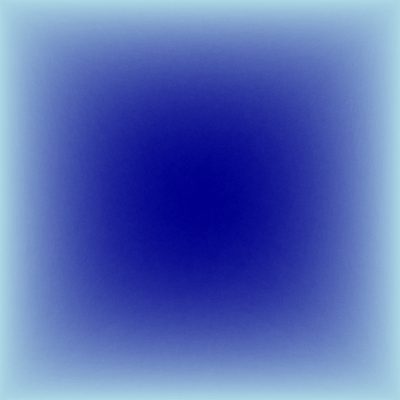
\includegraphics[width=\textwidth]{src/youtube/datashader/simple/fullgraph}
    \caption{Directly connected layout - Plot of the full graph}
    \label{fig:ds_fullgraph}
\end{figure}

%- - - - - - - - - - - - - - - - - - - - - - - - - - - - - - - - - - - - - - - -
\subsubsection{Plotting communities}
%- - - - - - - - - - - - - - - - - - - - - - - - - - - - - - - - - - - - - - - -



%-------------------------------------------------------------------------------
\newpage
\subsection{Plotting small graphs (igraph)}
%-------------------------------------------------------------------------------
%- - - - - - - - - - - - - - - - - - - - - - - - - - - - - - - - - - - - - - - -
\subsubsection{Goals and section overview}
%- - - - - - - - - - - - - - - - - - - - - - - - - - - - - - - - - - - - - - - -
\myparagraph{Goals}

\begin{enumerate}
  \item To show how to create a regular graph's plot, and consider the idea that its simplicity may make it harder to read
  \item To show how to create a graph plot with marked communities on it, and compare it to the regular plot in terms of ease of reading
  \item To show how to create a graph plot with marked communities that also shows the weight of its nodes, and compare this plot to the other two
\end{enumerate}

\myparagraph{Description}

In this section, I will show you how to plot a smaller (around 1000 nodes) portion of our graph using tools that are supported by igraph, in particular using its bindings to a C library called \improvement{citation needed} cairo. Since it is originally written in C and only provides an API that other languages can use, we will also have to use a package that will be able to connect python code to the C library itself. In this example, I'm using cairocffi as such package, hence the inclusion of \texttt{import cairocffi as cairo} in the starting import list. We have to import it as cairo, because otherwise igraph will attempt to use a different binding package, \texttt{pycairo}, which is quite outdated and can outright refuse to save vector images.

%- - - - - - - - - - - - - - - - - - - - - - - - - - - - - - - - - - - - - - - -
\subsubsection{Regular plot}
%- - - - - - - - - - - - - - - - - - - - - - - - - - - - - - - - - - - - - - - -
\myparagraph{Selecting vertices}

First thing that we have to do in this section is to select a subgraph for plotting. I have decided to settle on the subgraph of vertices with high degrees, because that meant that every node would be connected to many other nodes, and that can be a good example of how to deal with clutter on the plot.

In order to select this subgraph, you can use the \texttt{graph.vs.select(*args, **kwargs)} method in your graph. This method works differently based on what you pass it:\newline

\begin{enumerate}
  \item If you pass a list of integers into it \texttt{select([1,2,3])}, or skip the list and call \texttt{select(1,2,3)}, it will return vertices at those indexes
  \item If you pass a special keyword argument to it, it will select all nodes with a property that match that argument
  \item If you pass a function to it, it will call that function on every vertex and return all vertices that the function has returned \texttt{True} for
  \item If you don't pass anything into the function, it returns an empty list
\end{enumerate}

The select method has 8 special keyword arguments:
\begin{multicols}{2}
  \begin{itemize}
  \item \texttt{eq} - equal to
  \item \texttt{ne} - not equal to
  \item \texttt{lt} - less than
  \item \texttt{gt} - greater than
  \item \texttt{le} - less than or equal to
  \item \texttt{ge} - greater than or equal to
  \item \texttt{in} - value is in the given list
  \item \texttt{notin} - value is not in the given list
  \end{itemize}
\end{multicols}

Please note, that you have to include the name of your property before the special keyword: \texttt{graph.vs.select(age\_in=[19,20,21])}. You can see how I have used \texttt{gt} in the following example. The \texttt{\_degree} you see in front of it is a semi-private variable (since no variable is truly private in python) that keeps track of the degree of the vertex.

\listcode[src/youtube/hdg/1_selecting.py]{Selecting nodes for the subgraph}

\myparagraph{Styling the resulting plot}

There are many different options to choose from if you want to change how the graph appears on the screen. They are originally available as keyword arguments that you can pass to the \texttt{ig.plot()} function, but I advocate for putting all of those kwargs in a separate dictionary, \improvement{move save\_fname to the dictionary too} since it takes away from the dissaray of having to include many options into one function call.

In this paper I will mainly focus on the layout option, as well as gloss over a couple of settings connected to the size of the vertices and edges, but if after reading this you will want to learn more about them, you can call \texttt{help(ig.plot)} while in a python interpreter to see the function's docstring.

One of the most important arguments provided to us is the layout one, since it changes how nodes and edges are positioned in the resulting plot. It is possible to choose from the following layouts\footnote{Visual comparison is available on the pages \pageref{fig:hdg_c1}-\pageref{fig:hdg_c9}}:

\begin{multicols}{2}
  \begin{itemize}
  \item Circle layout
  \item Star layout
  \item Grid layout
  \item Fruchterman Reingold layout
  \item Fruchterman Reingold grid layout
  \item DrL layout
  \item Graphopt layout
  \item Kamada Kawai layout
  \item Sugiyama layout
  \item Random layout
  \item Large Graph layout
  \item Reingold Tilford layout (for trees)
  \item Bipartite layour (for 2-layer graphs)
  \end{itemize}
\end{multicols}

As you can see in the listing, other options are responsible for things like edge width, vertex size and shape, where to save the file, et cetera. The \texttt{bbox} argument is responsible for how big your final plot is going to be (in another words, it is declaring a limiting box on a figure that no vertex can cross). The \texttt{target} keyword argument is also very useful - it specifies the name of the file that your final chart will be stored in, and supports multiple file extentions (PDF, SVG, PNG).  In the next section I will also explain you how to add a color palette to the dictionary in order to distinguish the communities that we will detect.

\listcodecont[src/youtube/hdg/2_style_dict.py]{Creating a style dictionary}

\myparagraph{Plotting and saving the resulting plot to a file}

Since we have already constructed the keyword argument dictionary for the plot function, the rest becomes very clean and easy - just pass it to the function while remembering to unroll it to convert it to key-value pairs.

\listcodecont[src/youtube/hdg/3_plotting.py]{Plotting the image}

\begin{figure}[hb]
    \centering
    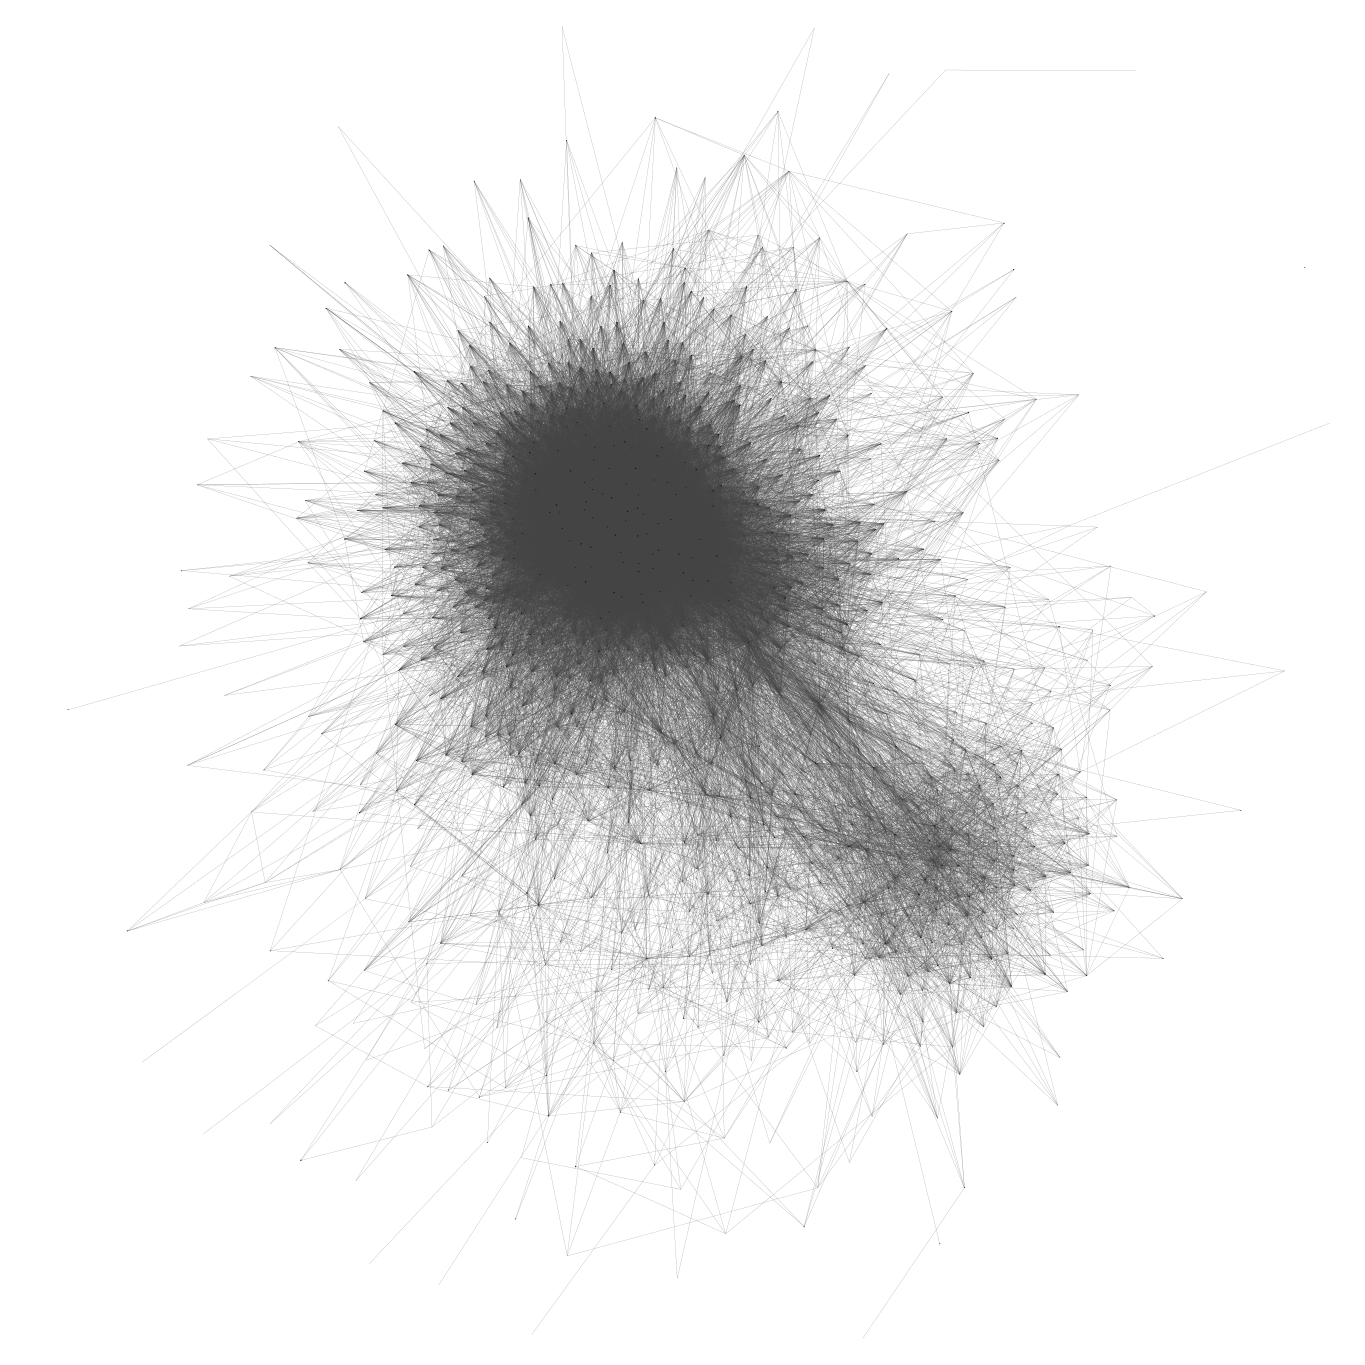
\includegraphics[width=\textwidth]{src/youtube/hdg/hdg_simple}
    \caption{Regular plot (Fruchterman Reingold layout)}
    \label{fig:hdg_simple}
\end{figure}

\myparagraph{Reviewing the results}

While igraph makes it quite easy to plot regular plots like these, they don't provide one with much insight into the data itself. While you could look at the picture made using the Fruchterman-Reingold layout, and detect two major communities in the network with a naked eye, other layouts aren't as simple to read. Furthermore, most of them look just black balls and are quite chaotic, which is a pretty large problem when dealing with plotting graphs.

Also, I'd like to note that while I would love to include the large graph layout in the following comparison, igraph (if its current version) refuses to draw anything when I use it.



\begin{multicols}{2}
  {\centering
  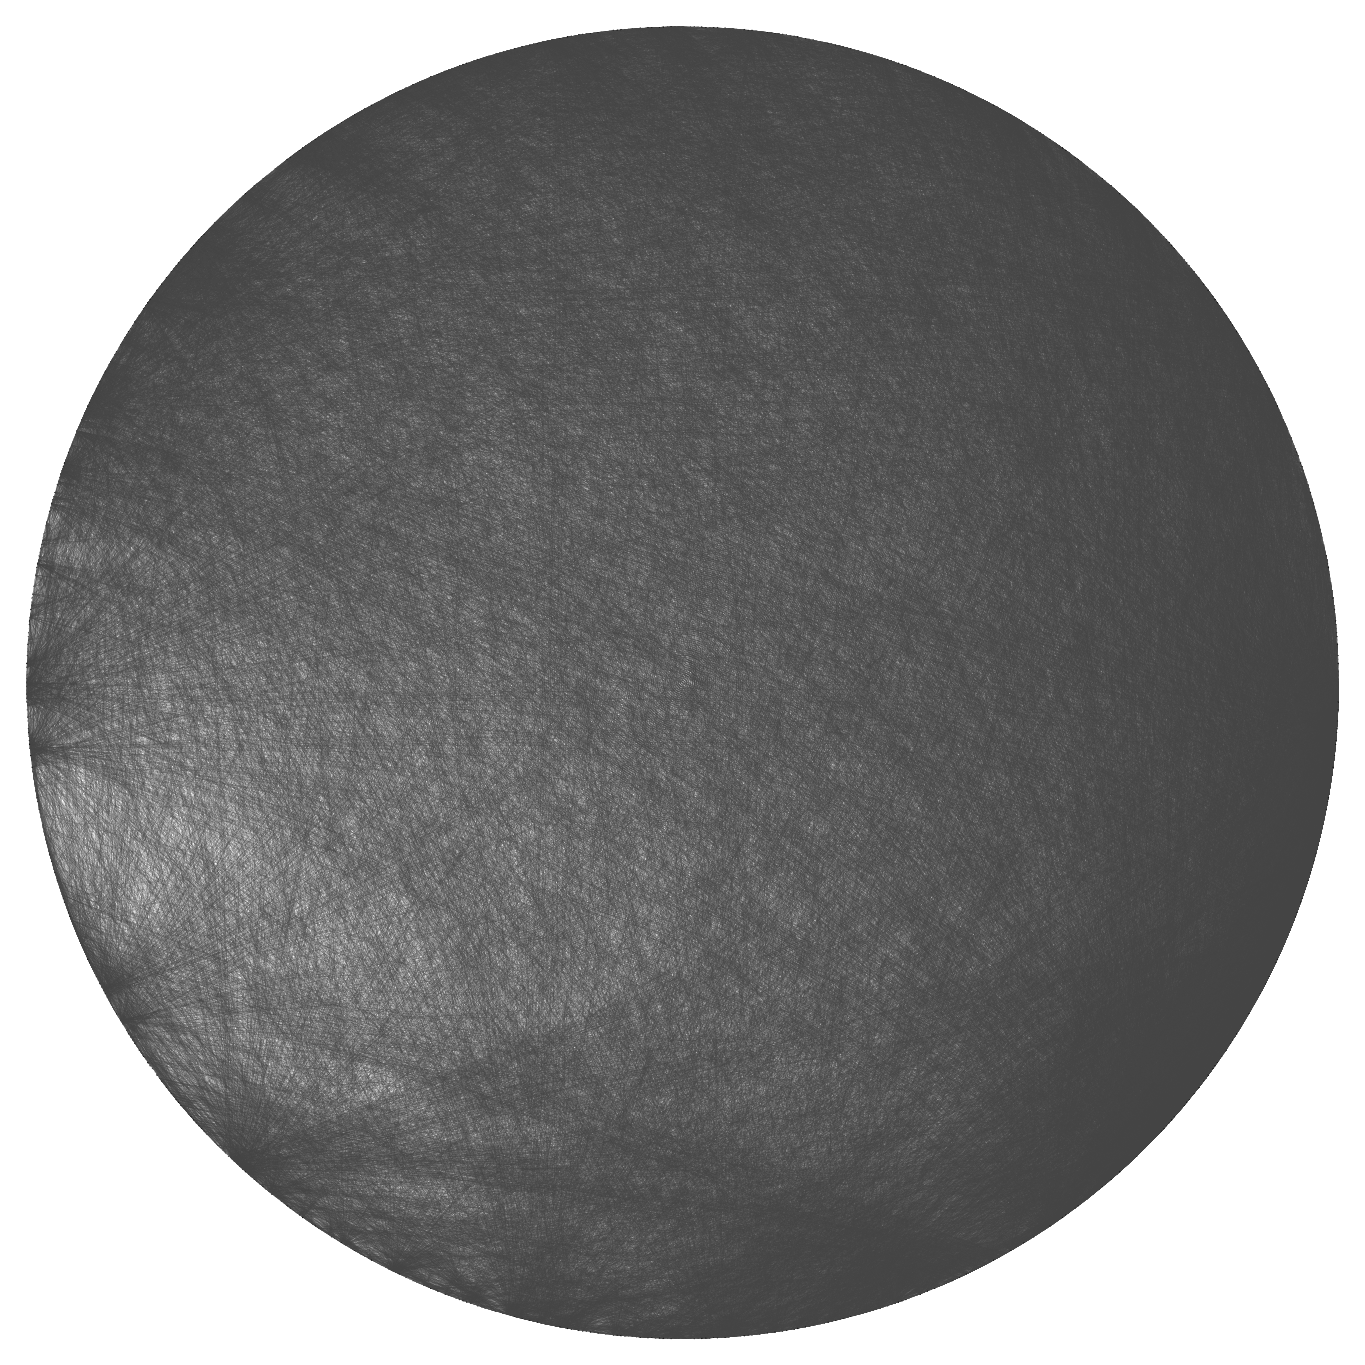
\includegraphics[width=\columnwidth]{src/youtube/hdg/comp/1_plot_crc}\\
  \captionof{figure}{Circular layout}
  \label{fig:hdg_c1}}
  {\centering
  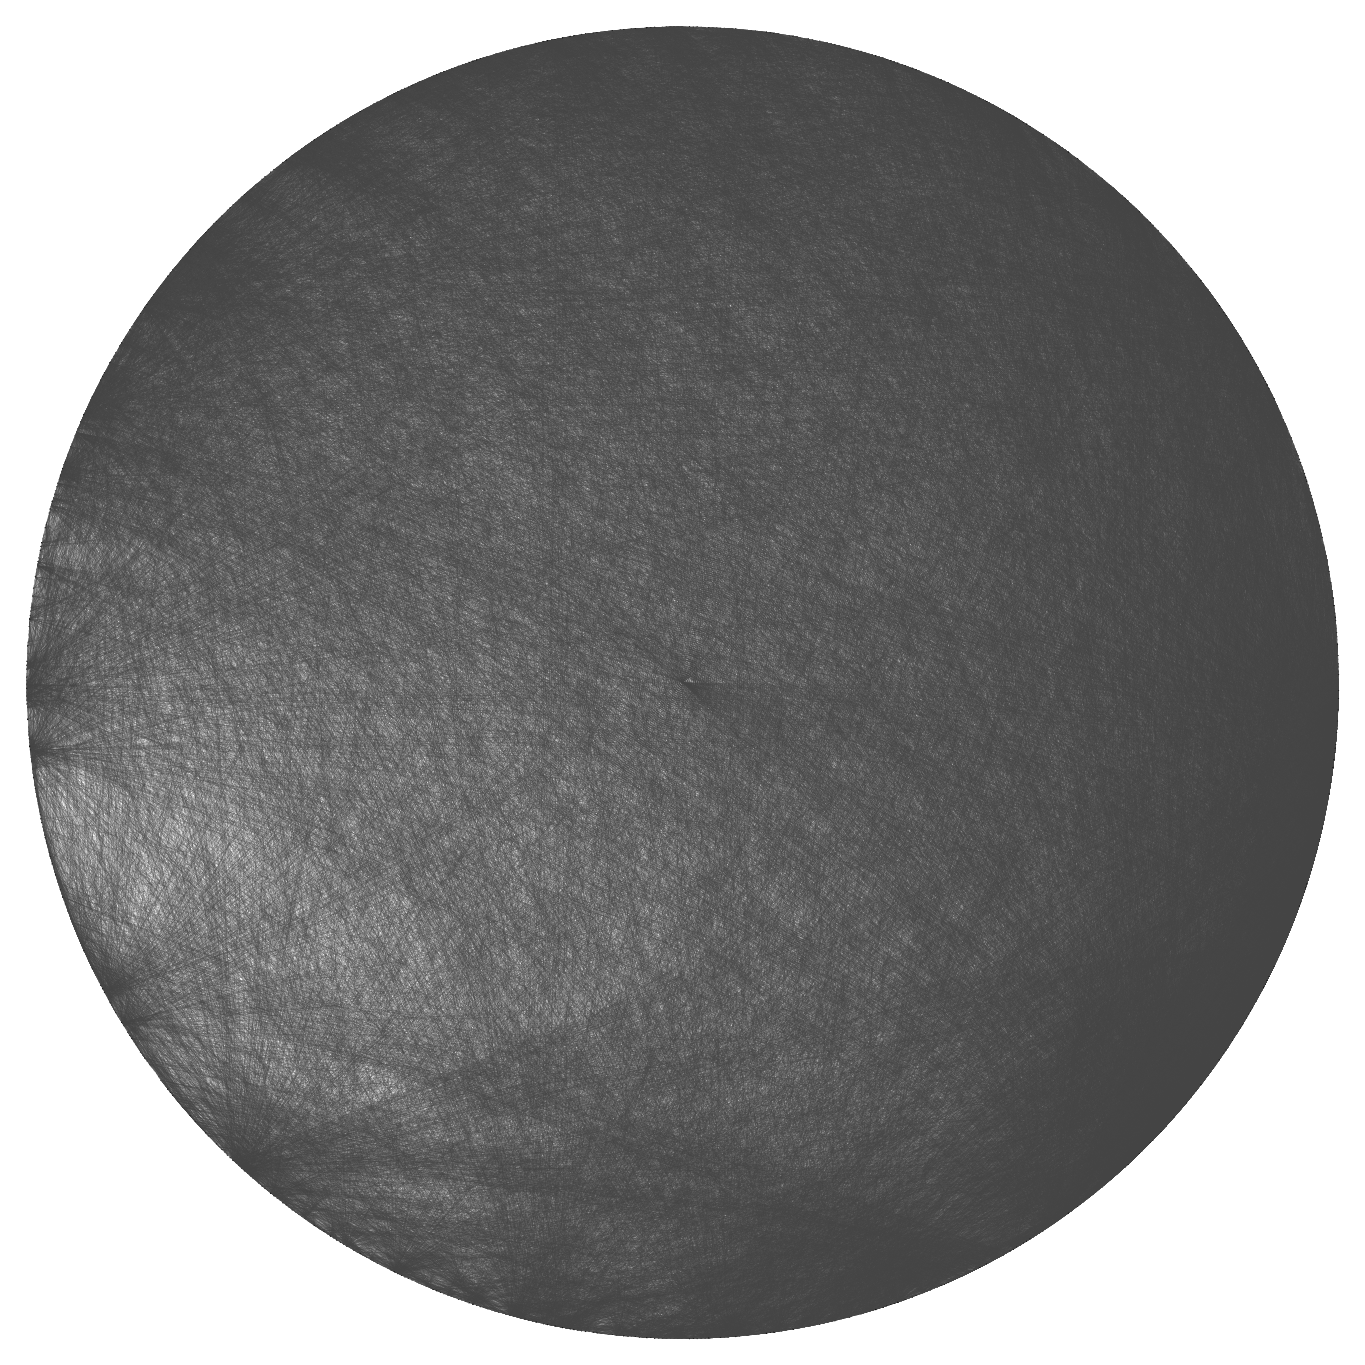
\includegraphics[width=\columnwidth]{src/youtube/hdg/comp/2_plot_str}\\
  \captionof{figure}{Star layout}
  \label{fig:hdg_c2}}
\end{multicols}

\begin{multicols}{2}
  {\centering
  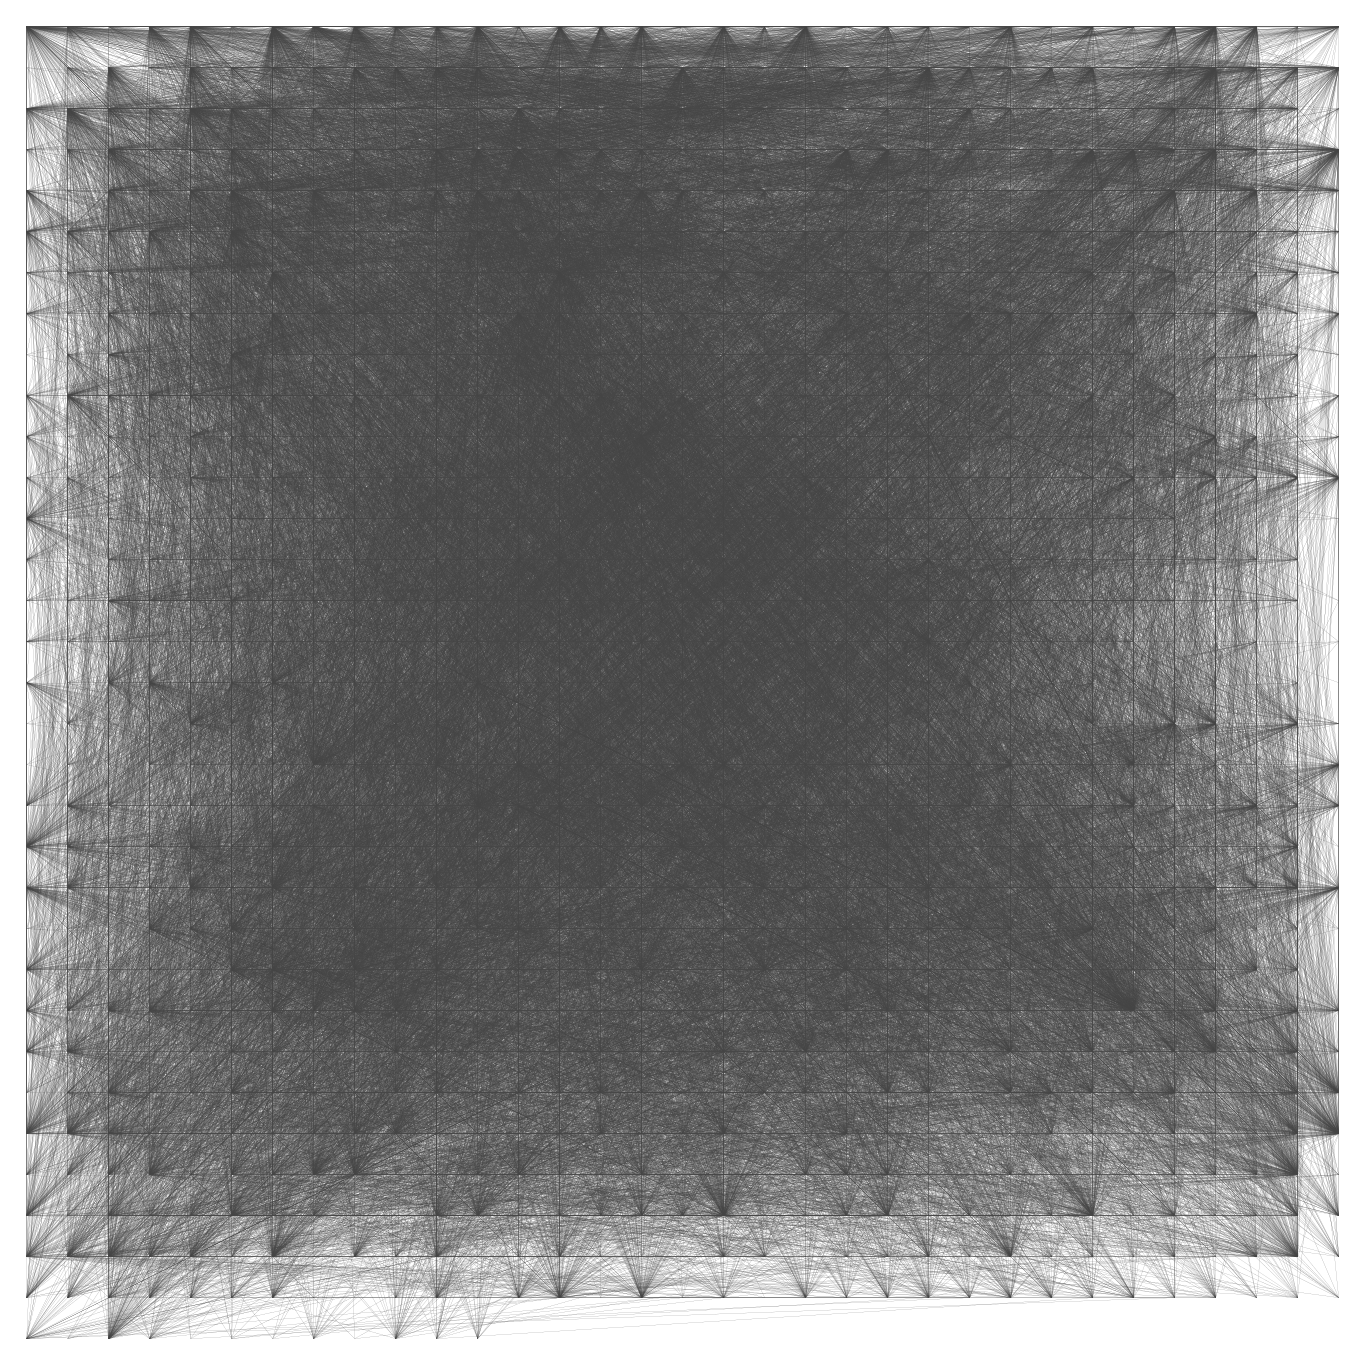
\includegraphics[width=\columnwidth]{src/youtube/hdg/comp/3_plot_grd}\\
  \captionof{figure}{Grid layout}
  \label{fig:hdg_c3}}
  {\centering
  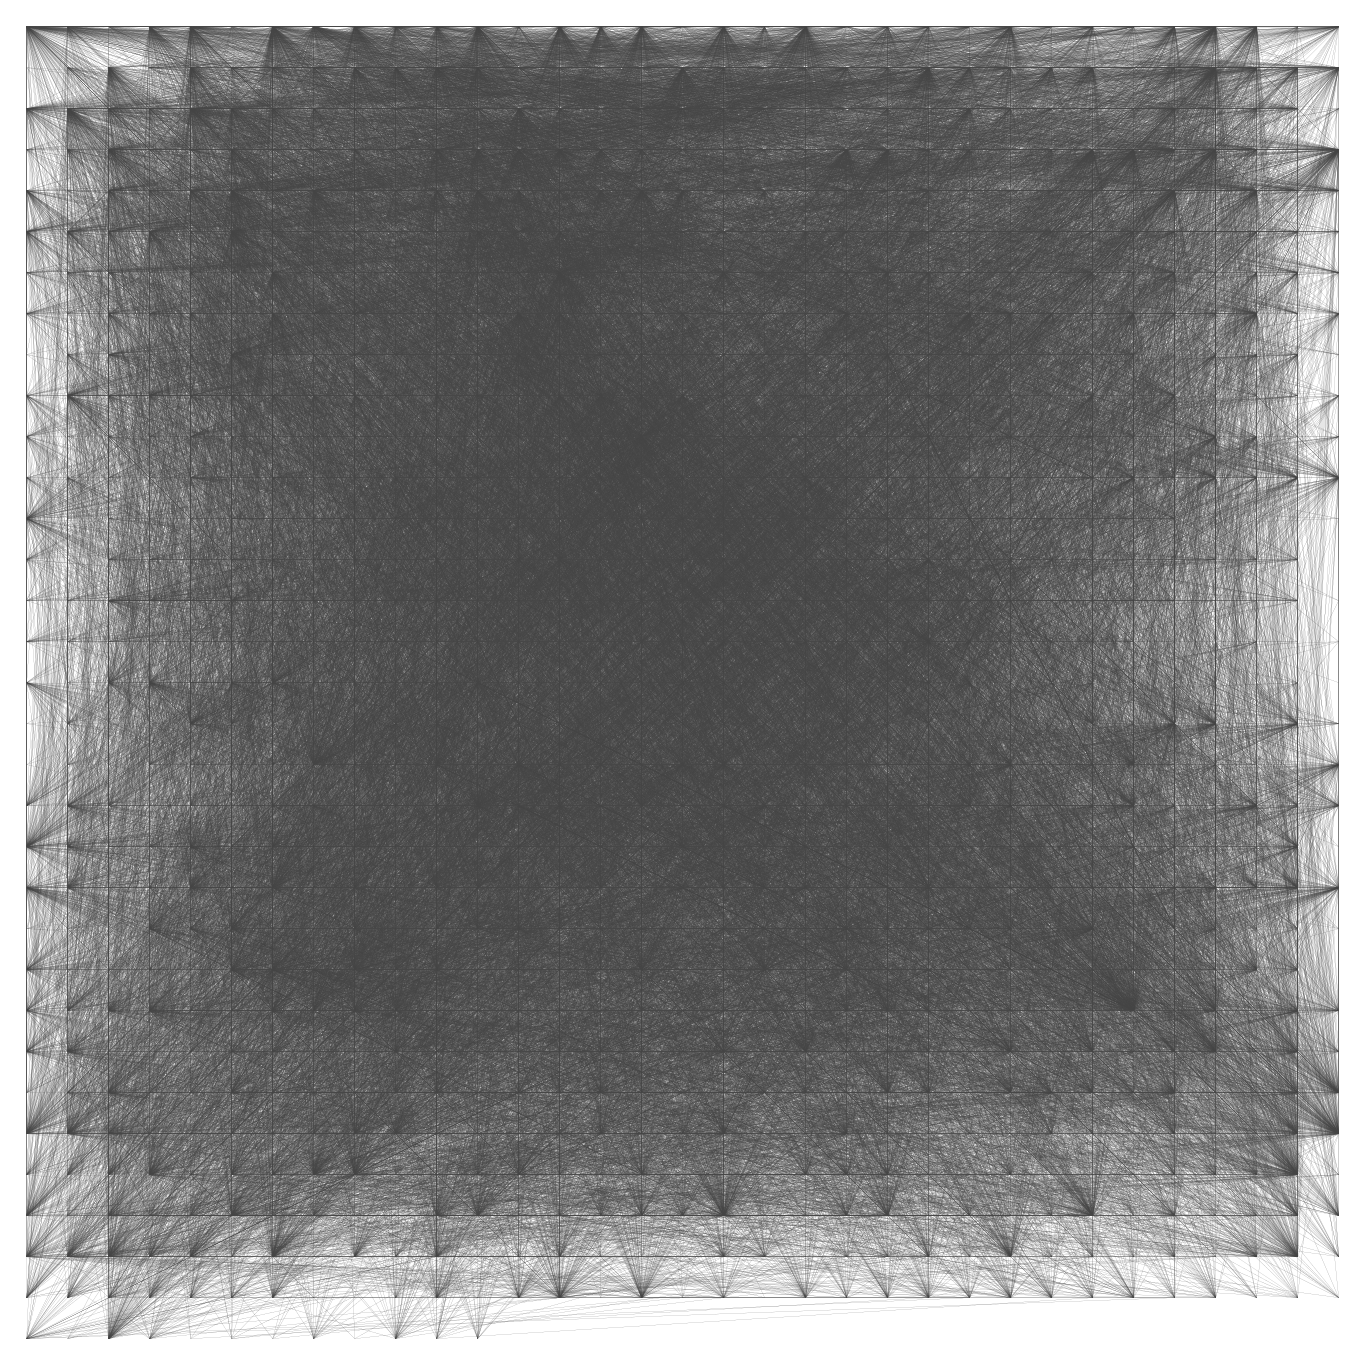
\includegraphics[width=\columnwidth]{src/youtube/hdg/comp/4_plot_frgrid}\\
  \captionof{figure}{Fruchterman Reingold grid layout}
  \label{fig:hdg_c4}}
\end{multicols}

\begin{multicols}{2}
  {\centering
  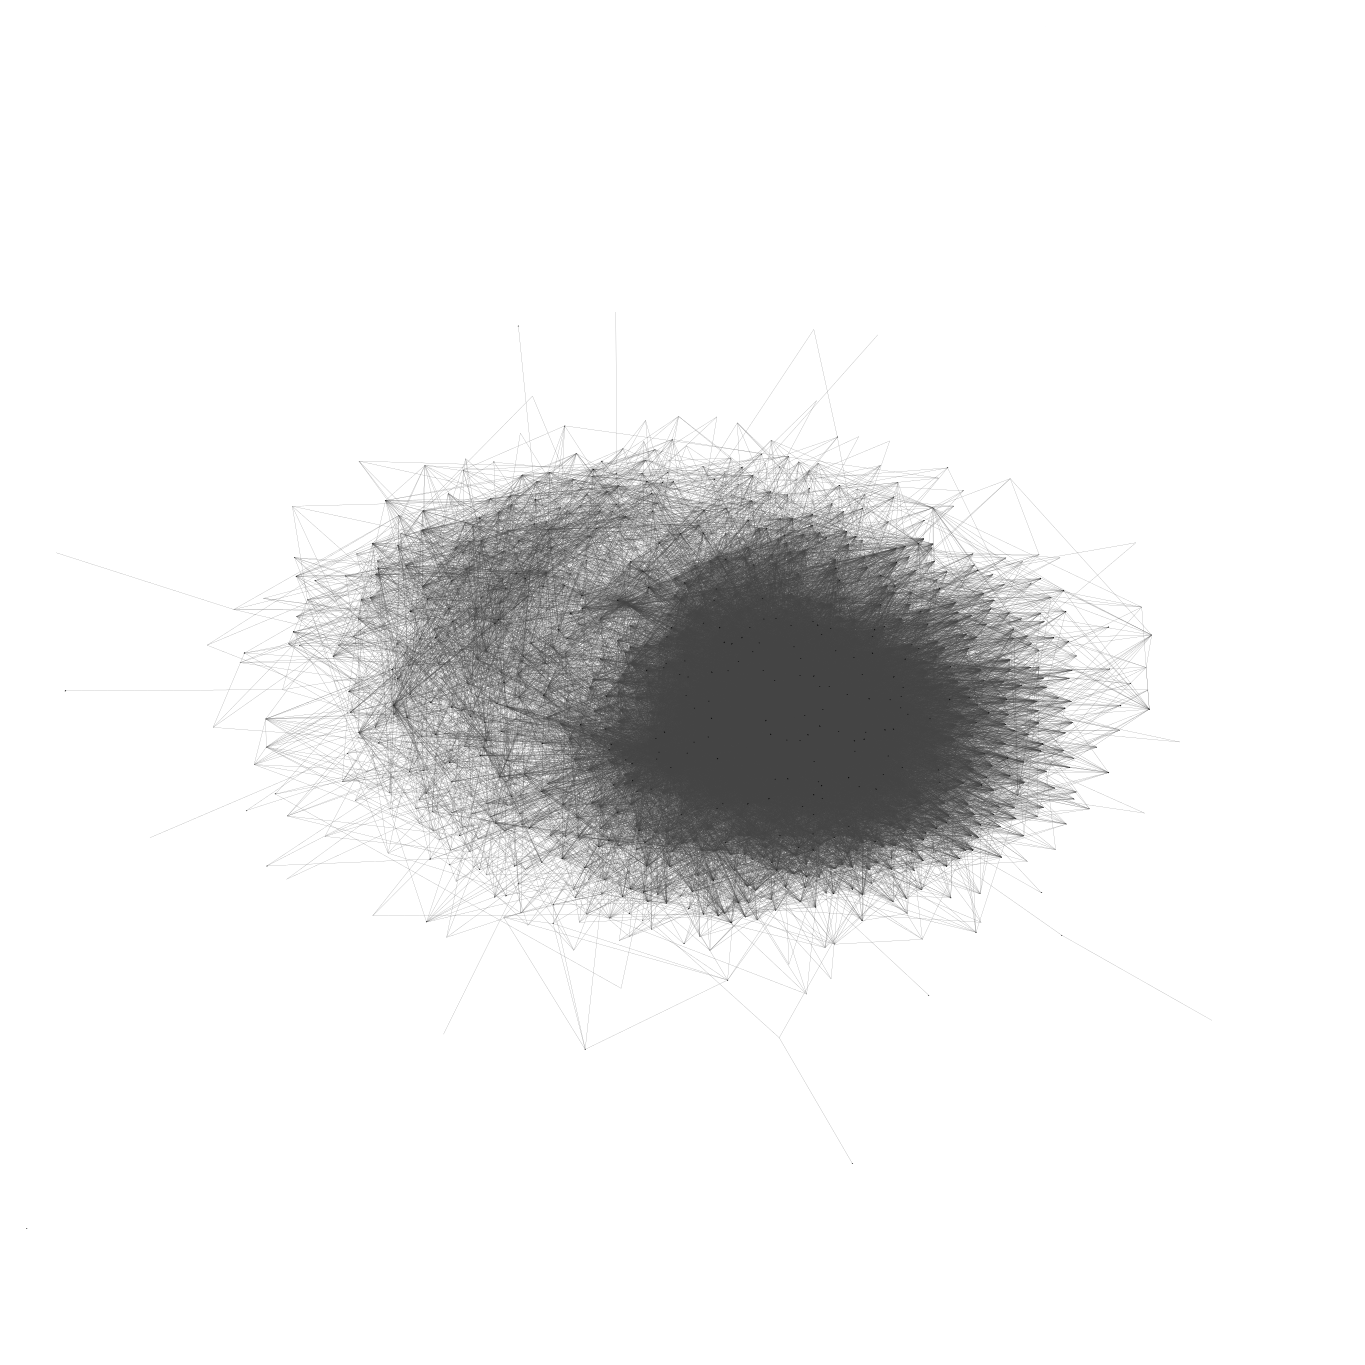
\includegraphics[width=\columnwidth]{src/youtube/hdg/comp/5_plot_kk}\\
  \captionof{figure}{Kamada Kawai layout}
  \label{fig:hdg_c5}}
  {\centering
  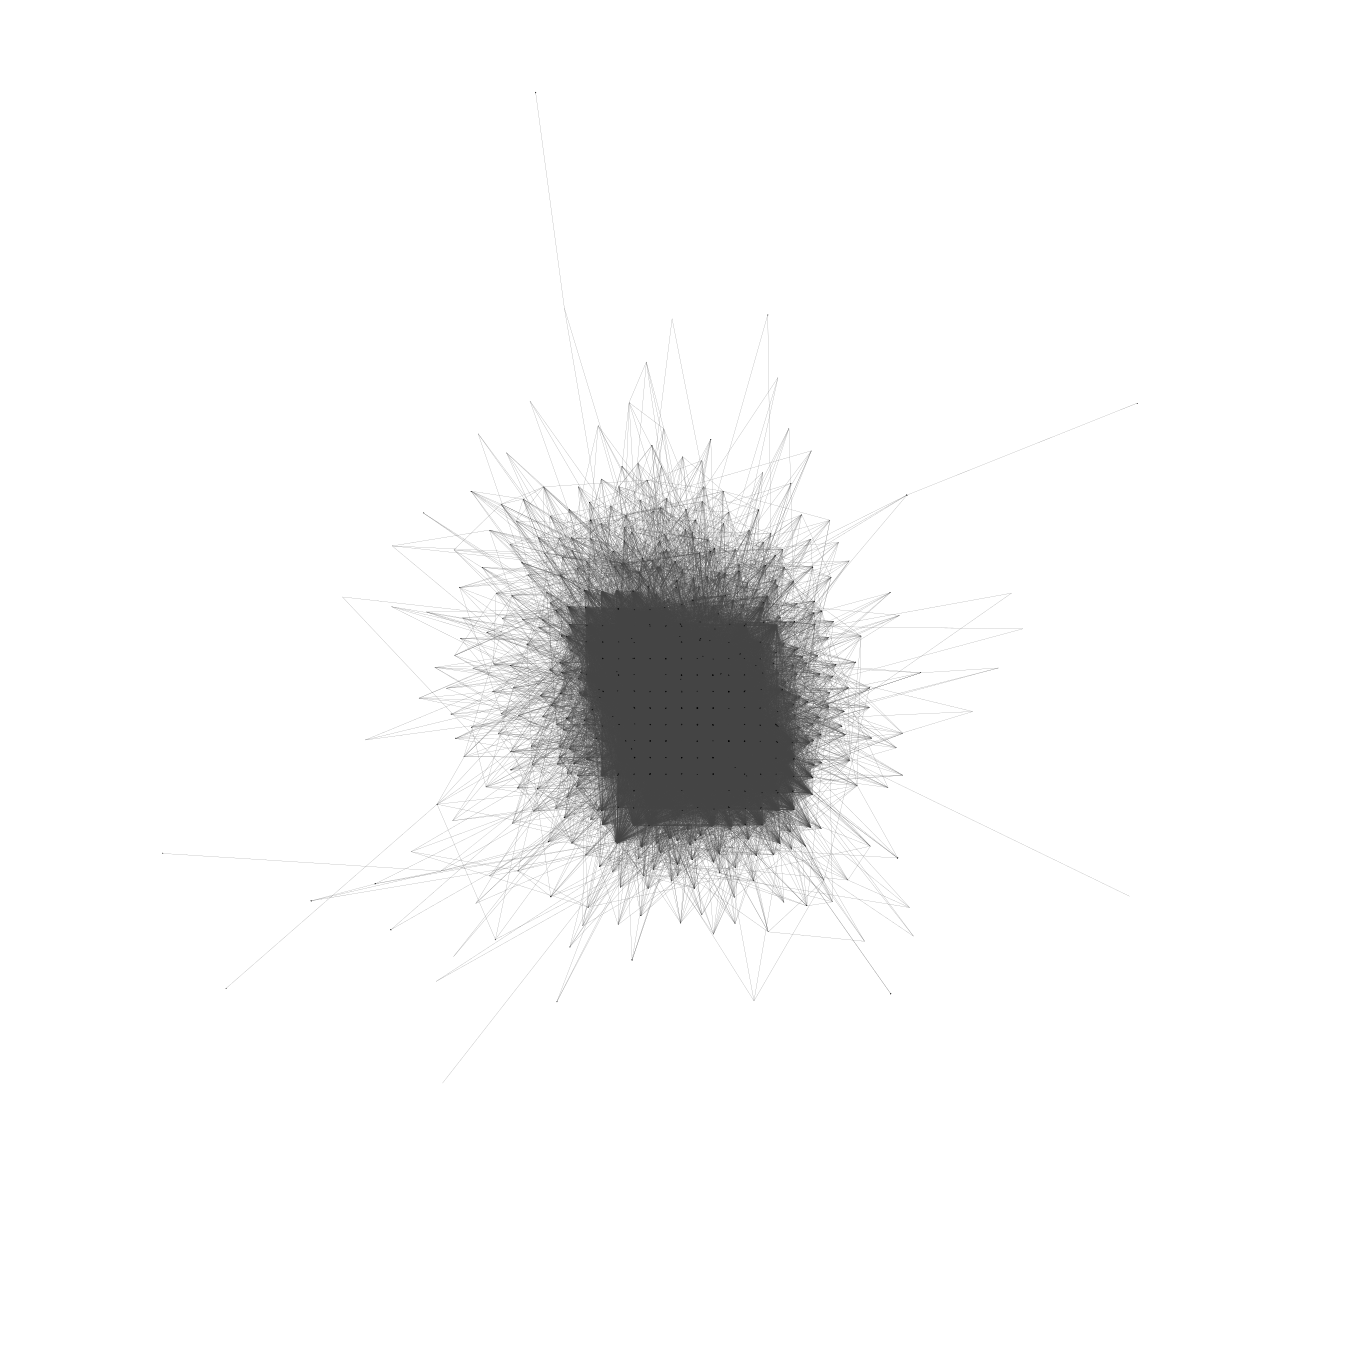
\includegraphics[width=\columnwidth]{src/youtube/hdg/comp/6_plot_ghopt}\\
  \captionof{figure}{Ghopt layout}
  \label{fig:hdg_c6}}
\end{multicols}

\begin{multicols}{2}
  {\centering
  
\includegraphics[width=\columnwidth]{src/youtube/hdg/comp/7_plot_drl}\\
  \captionof{figure}{DrL layout}
  \label{fig:hdg_c7}}
  {\centering
  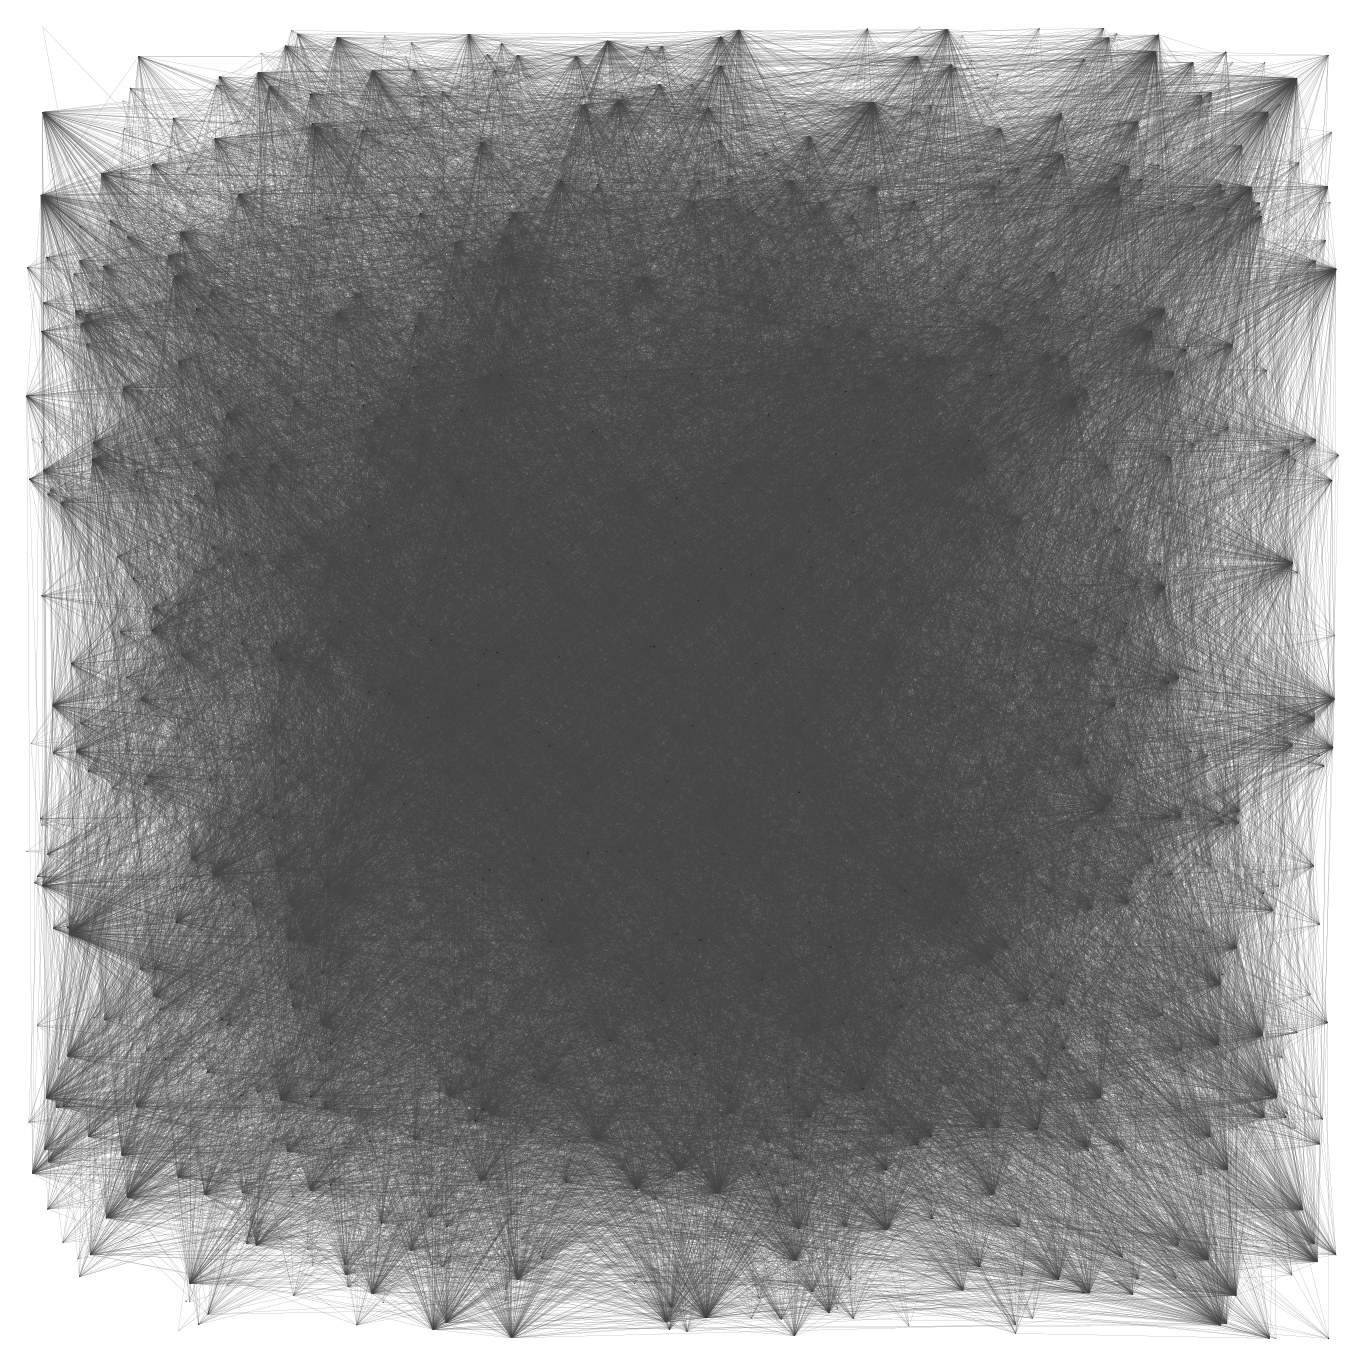
\includegraphics[width=\columnwidth]{src/youtube/hdg/comp/8_plot_random}\\
  \captionof{figure}{Random layout}
  \label{fig:hdg_c8}}
\end{multicols}

  {\centering
  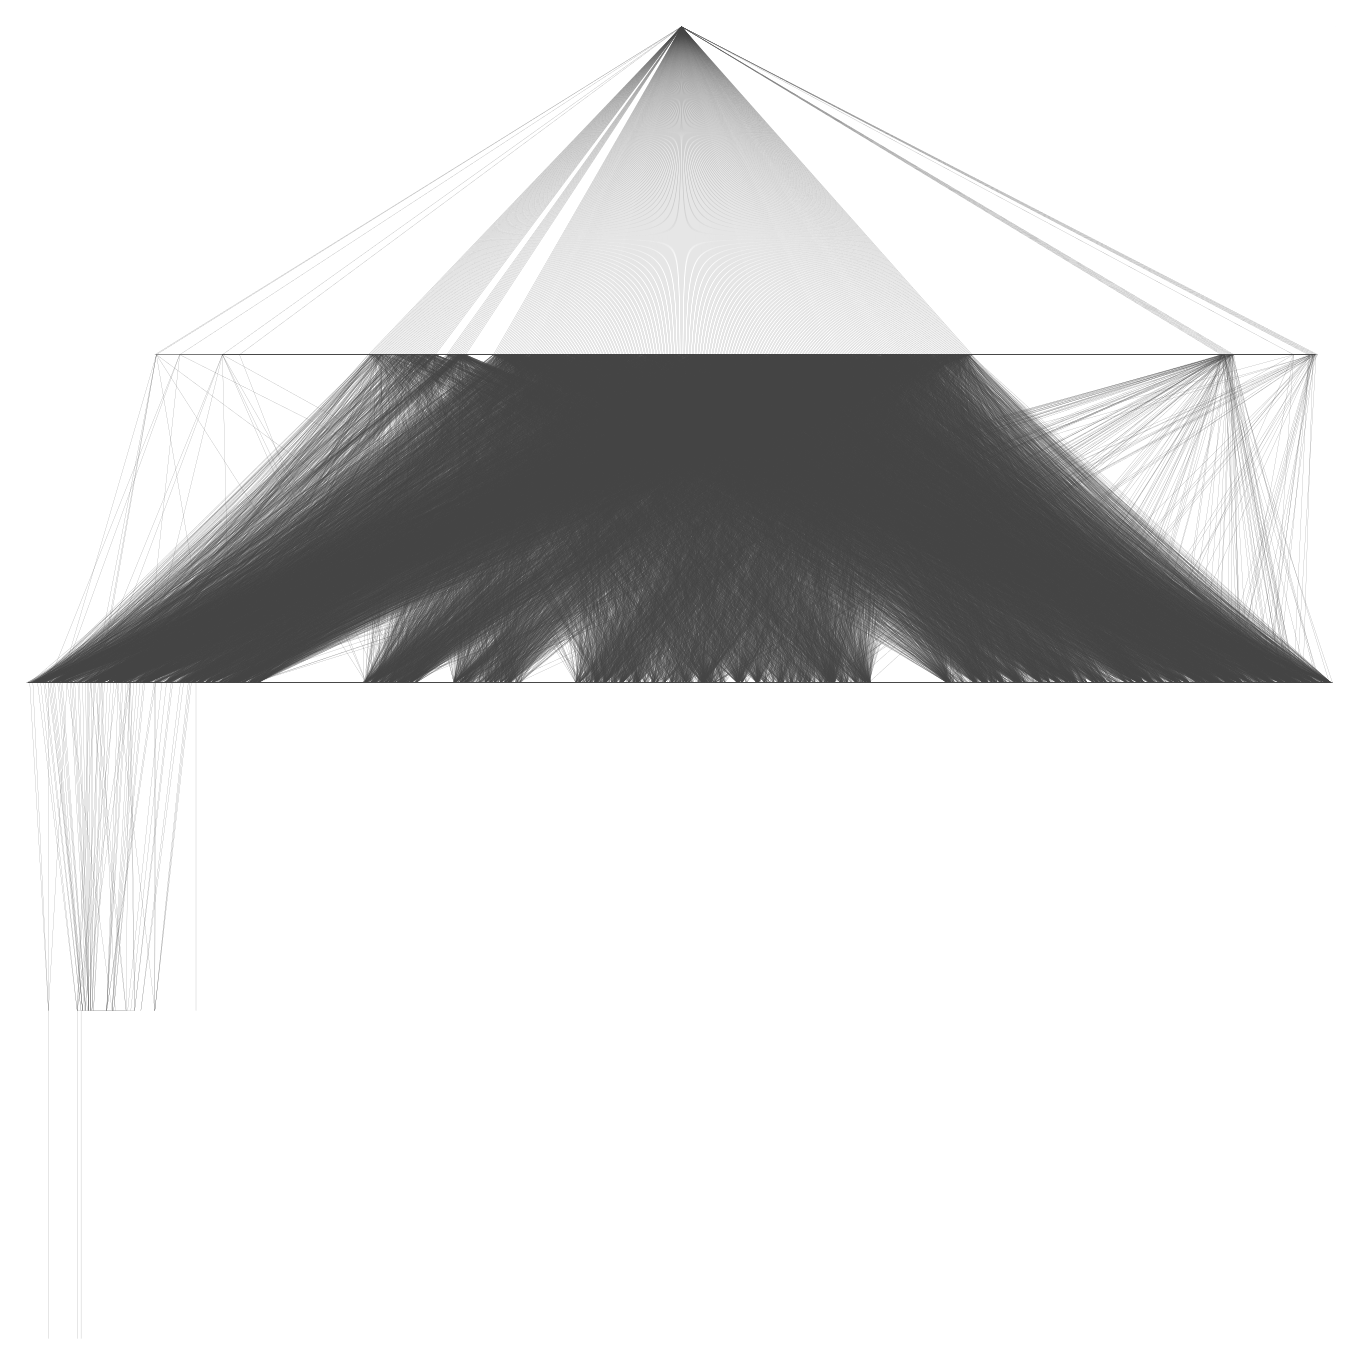
\includegraphics[width=\columnwidth]{src/youtube/hdg/comp/9_plot_sgy}
  \captionof{figure}{Sugiyama layout}
  \label{fig:hdg_c9}}

%- - - - - - - - - - - - - - - - - - - - - - - - - - - - - - - - - - - - - - - -
\newpage
\subsubsection{Community plot}
%- - - - - - - - - - - - - - - - - - - - - - - - - - - - - - - - - - - - - - - -
\myparagraph{Clustering the subgraph}

The size of the subgraph we're clustering is smaller than the one used in the datashader example, so using infomap right away without needing to cluster it with the louvain algorithm in advance is reasonable. In here I'm also storing the node's membership list into a variable, because we will need it later to color edges.

\listcode[src/youtube/hdg_com/1_clustering.py]{Using infomap to cluster the subgraph}

\myparagraph{Making communities visible}

There are a couple of ways to make communities in your graph more visible on the resulting plot. You could (1) use color to distinguish between them, (2) draw vertices from one community close to each other, (3) separate communities by drawing their boundaries, or (4) label each vertice with their community label. Some of those techniques are only effective when applied to very small graphs (like labeling), while other are a better fit for a medium-sized graph like the one used in this example.

In this example, I have decided to color all vertices within a community and edges between them using one color and to assign very heavy weights to them, and used a more neutral color for edges between vertices that belong to two different communities as well as assigning a very light weight to them. This guarantees that when I will run the fruchterman reingold layout algorithm, the communities will be pulled apart from each other, while vertices in a community will remain together.

As for colors, since the number of communities changed whenever I ran the infomap algorithm, I have decided to go with a randomized approach and just generate a random color for each community using a list comprehension and the \texttt{random.randint(min, max)} function that would give me a color-representing number that then would be converted to hex using the \texttt{06x} string format.

\listcodecont[src/youtube/hdg_com/2_initializing_colors.py]{Initializing color and weight lists}
\ \\
To assign color to a vertice in igraph, you can just add an attribute \textquotedblleft color\textquotedblright to the vertex, and igraph with cairo will fill that vetice with that color if it is in the pallette that you have to assign in the keyword argument (or style) dictionary. The enumerate function adds an id to the every member of an iterable that you pass into it, so I used it to get access to the community ID numbers, since the \texttt{comm}  variable is just a list of vertices. Then I proceeded to iterate through every vertice and assign a matching color to them.\\

\listcodecont[src/youtube/hdg_com/3_colors_looping_vert.py]{Assigning color to vertices}
\ \\
I did a very similar thing to the edges, except this time I have checked whether both of their ends are in one community and assigned different color and weights based on that.

\listcodecont[src/youtube/hdg_com/4_colors_looping_edge.py]{Assigning color to edges}

\myparagraph{Styling the resulting plot}

In order for igraph to be able to use a color, it has to be in it's palette. You can either use standard colors from the standard palette or create your own PrecalculatedPallette, passing the color list into the function (color can be specified using hex, rgb or their english names like \textquotedblleft red\textquotedblright). So, while the edges' and vertices' colors are decided based on their color attribute, the palette that those colors will be drawn from have to be specified in the style dictionary or as a regular keyword argument. You can also use the \texttt{mark\_groups} option if you either don't want to color the vertices or edges yourself or just want to make sure that every group is clearly delineated and is very visible\footnote{You can see how it looks on the pages \pageref{fig:hdg_com}-\pageref{fig:hdg_com_marked}}.

One more new thing in this code listing is the \texttt{edge\_order\_by} argument, and it is quite important for this example, since it determines the order that the edges are drawn in. So, if we order them by weight that means that the the gray edges between communities that have lighter weights will be drawn first, and the heavier and more colorful edges inside of the communities will be drawn on top of them.

\listcodecont[src/youtube/hdg_com/5_styling_prop.py]{Styling using graph properties}

\listcodecont[src/youtube/hdg_com/6_style_dict.py]{Styling using a style dict}

\myparagraph{Plotting and reviewing the results}

\listcodecont[src/youtube/hdg_com/7_plotting.py]{Saving the plot to a file}

Looking at this plot, I find that the clear separation between groups and their coloring makes them easier to distinguish from each other. And while the delineated plot can be less pretty for some people, it separates the communities even more than the regular coloring does, and adds boundaries that make even smallest groups of 2-3 vertices visible due to the bold lines connecting them. The problem with that plot is that the boundaries that separate the groups are drawn first, which makes them being crossed over by the edges that connect different communities. While that thing can be changed by inheriting from some parts \improvement{insert accurate data here} of the cairo library and rewriting them, I can't help but think that it's done intentially, just so you could actually see the edges that connect the communities.

Anyway, adding some kind of order with the groups and colors is in my mind an improvement compared to the seemingly random balls of black lines that were generated in the last section.

Some could also argue that some of the colors aren't mixed well, to which I can only respond by reccomending others to select colors they would like to see on a plot.\improvement{Change the color from random to a normal list?}

\begin{figure}[p]
    \centering
    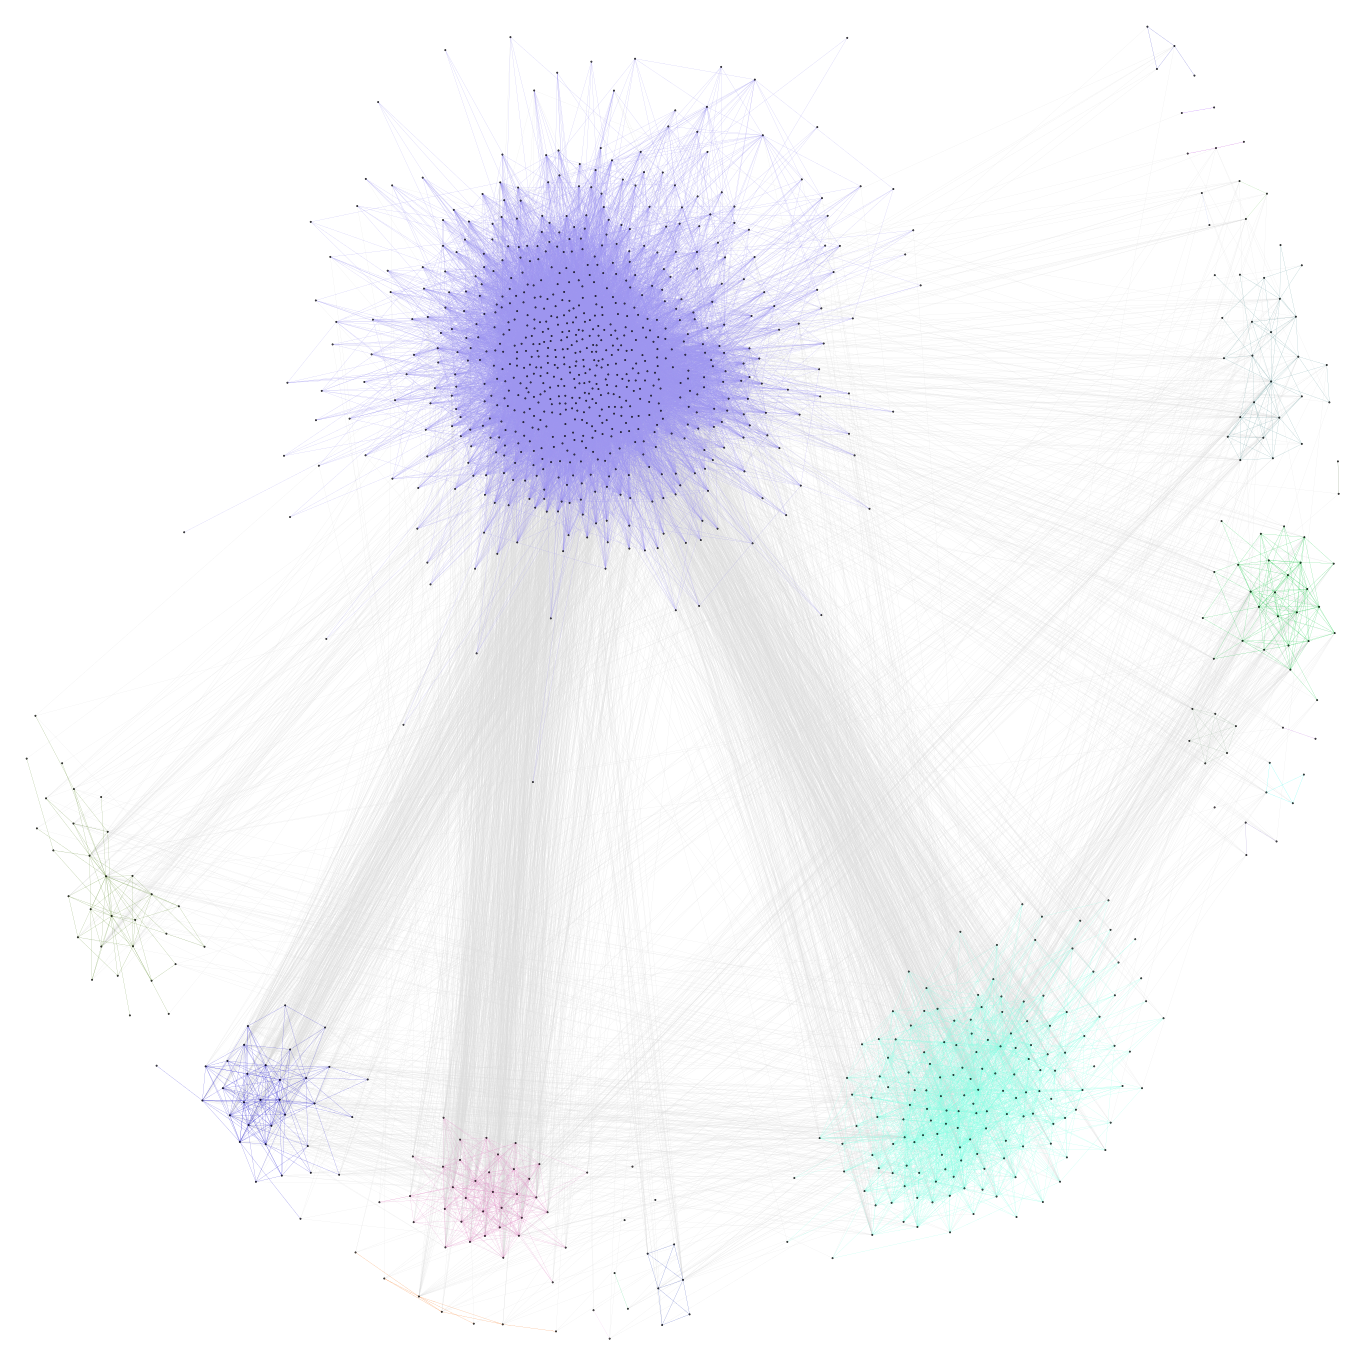
\includegraphics[width=\textwidth]{src/youtube/hdg_com/hdg_com}
    \caption{Community plot - Fruchterman Reingold layout}
    \label{fig:hdg_com}
\end{figure}

\begin{figure}[p]
    \centering
    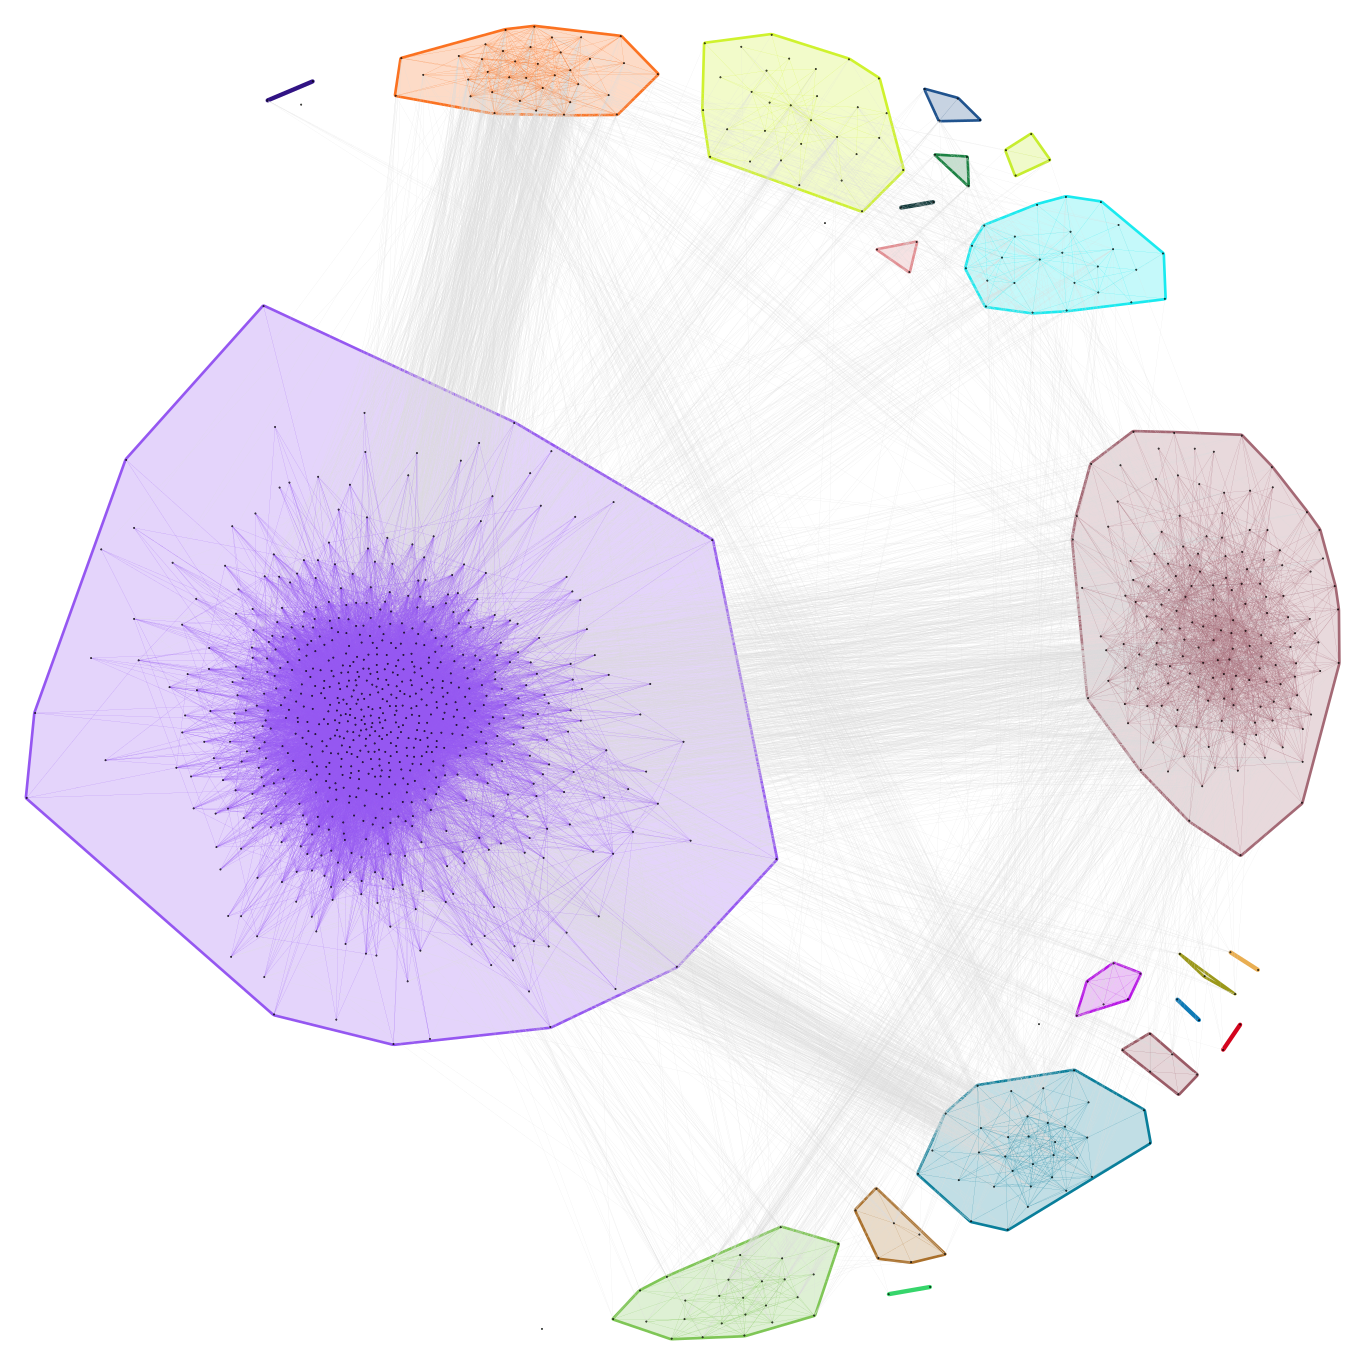
\includegraphics[width=\textwidth]{src/youtube/hdg_com/hdg_com_marked}
    \caption{Community plot - delineated groups - Fruchterman Reingold layout}
    \label{fig:hdg_com_marked}
\end{figure}

%- - - - - - - - - - - - - - - - - - - - - - - - - - - - - - - - - - - - - - - -
\newpage
\subsubsection{Weighted community plot}
%- - - - - - - - - - - - - - - - - - - - - - - - - - - - - - - - - - - - - - - -
\myparagraph{Pagerank application}

Pagerank \improvement{cite} is an algorithm developed by google. It uses a number of links to a specific vertex (originally a webpage) to evaluate their importance. This metric is used as the weight of the vertices in this example. The pagerank implementation in the igraph package already auto assigns the weight, so you don't have to do that yourself.

\listcode[src/youtube/hdg_weighted/1_pagerank.py]{Using pagerank to assign weights to vertices}

\myparagraph{Style dictionary}

Style dictionary for the weighted graph is very similar to the one that was used to create the community plot, with an additions of weights as a keyword argument to pass to the fruchterman reingold layout and vertice size now depending on it's weight instead of being constant. As you can see from the code listing, the \texttt{vertex\_size} requires either a constant number or a iterable of all vertices' weights.

\listcodecont[src/youtube/hdg_weighted/2_style_dict.py]{Styling using a style dict}

%
\myparagraph{Plotting and reviewing results}

\listcodecont[src/youtube/hdg_weighted/3_plotting.py]{Saving the plot to a file}

Comparing this plot to the previous two, this clearly presents the most information out of the three. If in the first section we had to only deal with the vertices and edges themselves, now we not only have communities of vertices that should be grouped, we also have different sizes of vertices inside those communities. While pagerank is an algorithm that always values nodes with more connection higher, thus making the violet community the most prominent group, if this chart was made using a different data set it could reveal something like the least populated community being the most important or something among those lines.


\begin{figure}
    \centering
    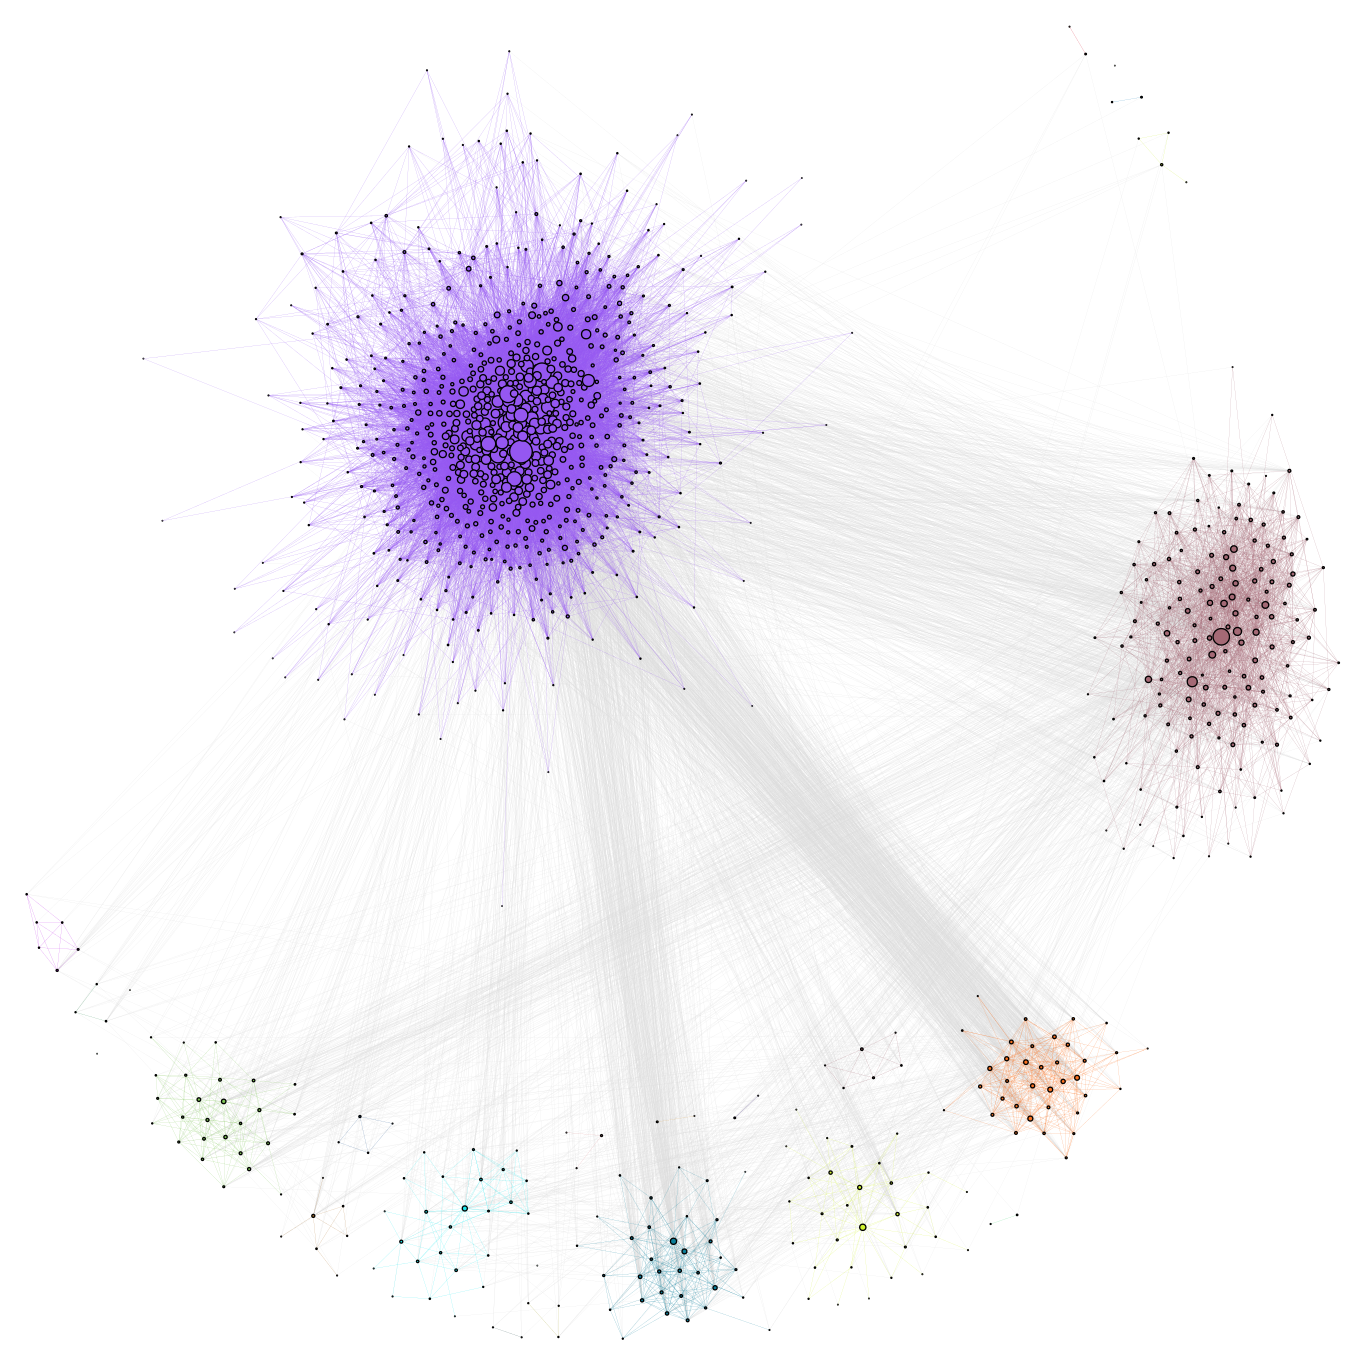
\includegraphics[width=\textwidth]{src/youtube/hdg_weighted/hdg_pg_fg}
    \caption{Weighted plot - Fruchterman Reingold layout}
    \label{fig:hdg_pg_fg}
\end{figure}

\begin{figure}
    \centering
    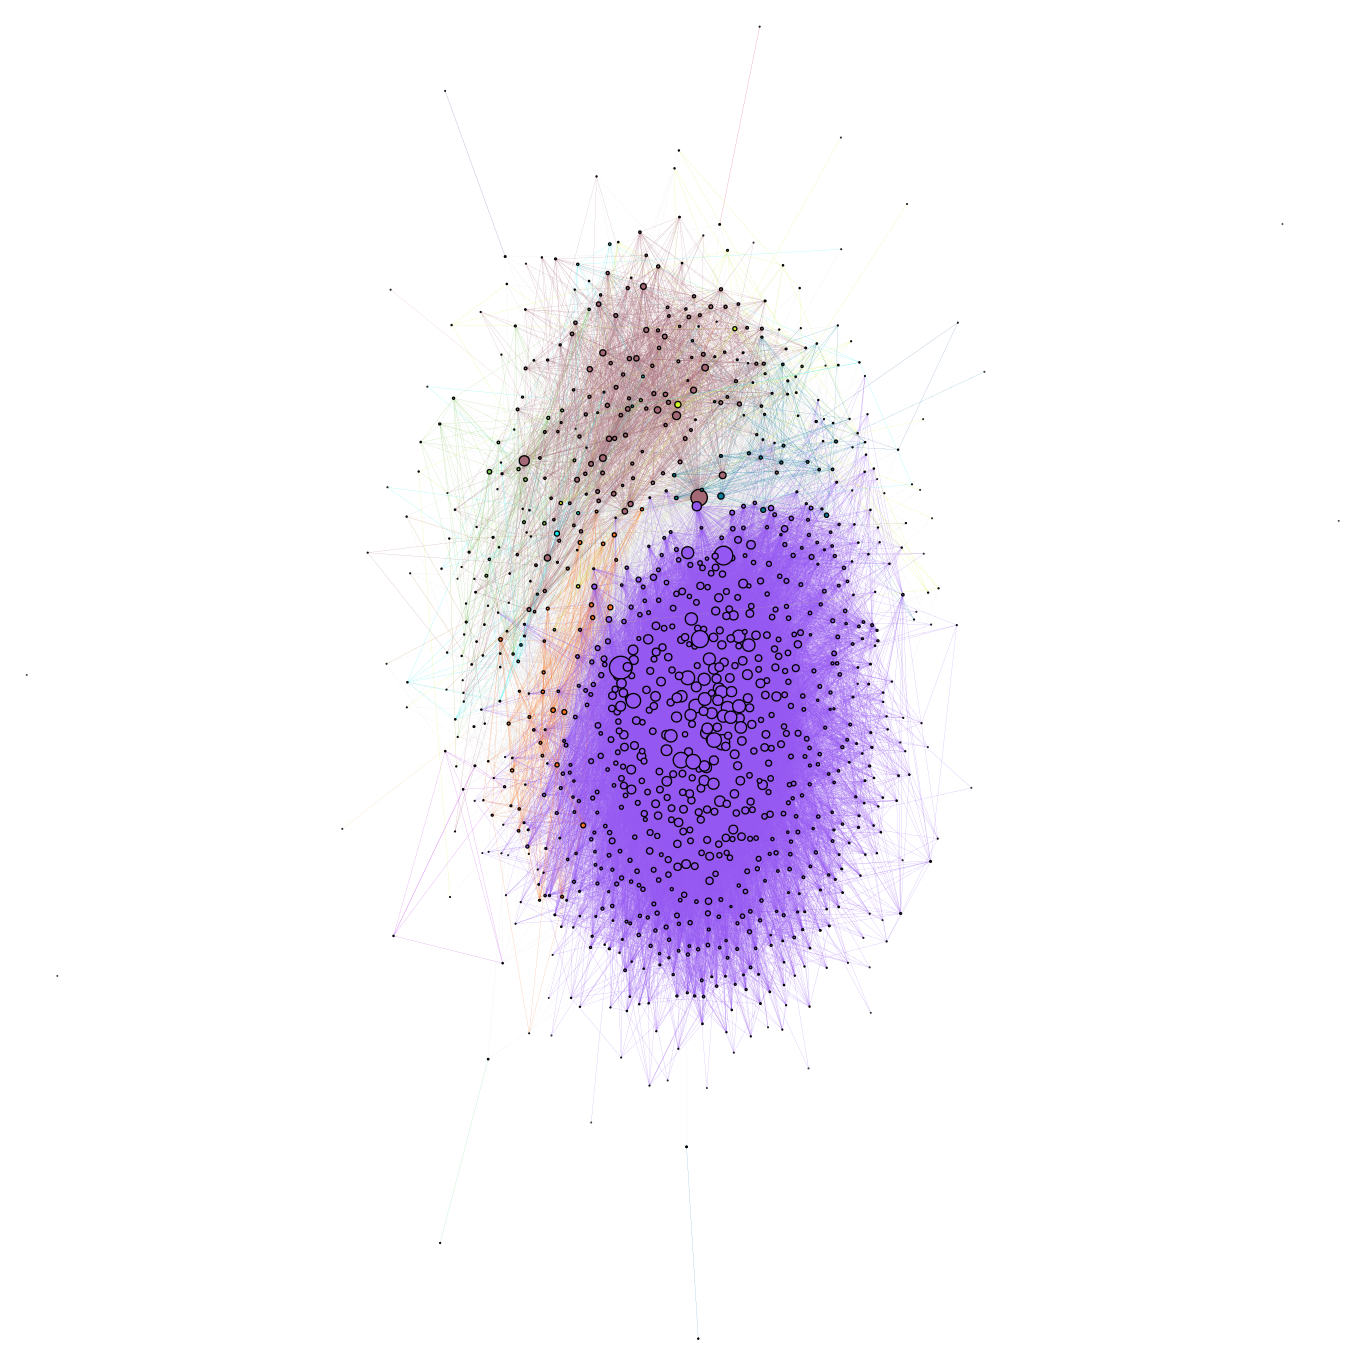
\includegraphics[width=\textwidth]{src/youtube/hdg_weighted/hdg_pg_kawai}
    \caption{Weighted plot - Kamada Kawai layout}
    \label{fig:hdg_pg_kawai}
\end{figure}



%===============================================================================
\newpage
\section{GEODATA ANALYSIS}
%===============================================================================

%-------------------------------------------------------------------------------
\subsection{Project Overview}
%-------------------------------------------------------------------------------
\begin{easylist}
# Goals
## to show how to deal with geodata in python
# Plots
## KPI per country (Basemap)
 ## Plot - Chikago Taxi (datashader)
\end{easylist}


%===============================================================================
\newpage
\section{CONCLUSION}
%===============================================================================

Include data types that we omit - biological data, food data, describe what you'd like for others to research.

% Literature references
\newpage
\nocite{*}
\bibliographystyle{unsrt}
\bibliography{references}

\end{document}
